实际项目中使用编程语言,是学习语言的一个步骤。有时,本书中的简单例子可能采用不同的方法,或者在实际程序中面临许多困难。理论需要与实践相结合。与学习语法、解决书本上的问题或理解书本上一些简单的例子不同,当创建实际的应用程序时,我们会面临一系列不同的挑战,有时书籍缺乏理论来支持实际问题。 \par
本章中,我们将尝试梳理C++实际编程的知识,这将帮助你更好地处理实际的应用程序。复杂的项目需要大量的思考和设计。有时候,因为开发者在开发之初做出了糟糕的设计选择,所以需要从头开始重写项目。本章描述了软件的设计过程。读者将了解为项目构建架构的步骤。\par
本章中,我们将了解以下内容: \par

\begin{itemize}
	\item 了解项目开发周期
	\item 设计模式及应用
	\item 领域驱动设计
	\item 设计一个Amazon的克隆版本作为一个真实项目的例子
\end{itemize}

\noindent\textbf{}\ \par
\textbf{编译器要求} \ \par
g++编译器需要添加编译选项 \texttt{-std=c++2a} 来编译本章的代码。可以从这里获取本章的源码文件:https:/​/github.​com/PacktPublishing/Expert-CPP \par

\noindent\textbf{}\ \par
\textbf{项目开发周期} \ \par
当处理一个问题时,应该仔细考虑需求分析的过程。项目开发中最大的错误之一是,在开始编码时没有对问题本身进行彻底的分析。 \par
想象一下这样一个场景,你的任务是创建一个计算器,允许用户对数字进行算术计算的简单工具。假设你奇迹般地按时完成了项目并发布了程序。现在,用户开始使用计算器,他们迟早会发现他们的计算结果不会超过整数的最大值。当他们抱怨这个问题时,就可以准备用可靠的编码来辩解,比如:它是因为在计算中使用了int数据类型。这对于你和你的程序员伙伴来说是完全可以理解的,但是最终用户就是不能接受你的观点。他们想要一个能够对大数字求和的工具,否则,他们根本不会使用你的程序。开始开发下一个版本的计算器时,将使用长数或甚至自定义实现的大数。当你自豪的将第二版程序交付给等待已久的用户时,用户可能会抱怨没有找到数字的对数或指数的功能。这就令人生畏了,因为可能会有越来越多的特性请求和越来越多的抱怨。 \par
虽然这个例子有点简单,但它完全涵盖了现实世界中经常发生的事情。即使开发者实现了程序的所有特性,并且正在考虑休假,用户也会开始抱怨程序中的错误。结果表明,有几种情况下,计算器的行为异常,没有给出或给出了错误的结果。迟早,您会意识到,在将程序发布给大众之前,需要的是适当的测试。 \par
我们将涉及在实际项目中工作时应该考虑的主题。当开始一个新项目时,应该考虑以下步骤: \par

\begin{enumerate}
	\item 需求收集和分析
	\item 创建规范
	\item 设计和测试计划
	\item 编码
	\item 测试和稳定性
	\item 发布和维护
\end{enumerate}

前面的步骤并不是针对每个项目都固定的,应该认为是每个软件开发团队为了实现成功的产品发布而应该完成的最低要求。现实中,大部分的步骤都被省略了,因为在IT领域的每个人都缺乏一件东西——时间。但是,强烈建议遵循上述步骤,因为从长远来看,它会节省更多的时间。 \par

\noindent\textbf{}\ \par
\textbf{需求收集和分析} \ \par
这是创建稳定产品的最关键的一步。开发者不能按时完成任务,或在代码中留下大量bug的一个最普遍的原因是缺乏对项目的完整理解。 \par
The domain knowledge is so important that it shouldn't be omitted 在任何情况下,你可能会很幸运地开发与你非常了解的东西相关的项目。然而,你应该考虑到不是每个人都像你一样幸运。 \par
假设您正在进行一个项目,该项目将自动分析和报告某个公司的股票交易信息。现在想象一下,你对股票和股票交易一无所知。你不知道熊市或牛市,交易的局限性等等。你将如何成功地完成这个项目? \par
即使您了解股票市场和交易,您也可能不知道您的下一个大型项目域。如果你的任务是设计和执行(有或没有团队)一个控制城市气象站的项目,那该怎么办?当你开始这个项目时,你首先要做什么? \par
你肯定应该从需求收集和分析开始。这只是一个涉及到与客户沟通和问很多关于项目的问题的过程。如果你在一家产品公司工作,而不是与任何客户打交道,那么项目经理就应该视为客户。即使这个项目是你的想法,你是独自工作,你也应该把自己当成客户,尽管这听起来可能有些荒谬,但你应该问自己很多问题(关于这个项目)。 \par
假设我们将征服电子商务,并希望发布一种产品,最终将在自己的业务领域击败市场鲨鱼。受欢迎和成功的电子商务市场有亚马逊、eBay、阿里巴巴等。我们应该把这个问题表述为,编写自己的Amazon版本。我们应该如何收集这个项目的需求? \par
首先,我们应该列出所有我们应该实现的功能,然后我们将优先级排序。例如,对于Amazon的项目,我们可能会得到以下特性列表: \par

\begin{itemize}
	\item 创建产品
	\item 展示产品
	\item 购买产品
	\item 修改产品的信息
	\item 删除产品
	\item 通过名称、价格范围和重量搜索产品
	\item 每隔一段时间通过电子邮件告知用户产品的可用性
\end{itemize}

应该尽可能详细地描述功能,这将为开发人员解决问题。例如,创建产品应该由项目管理员或任何用户完成。如果用户可以创建产品,则应该有限制。用户可能会错误地在我们的系统中创建数百个产品,以增加他们唯一产品的可见性。 \par
与客户沟通的过程中,应陈述、讨论和最终确定细节。如果项目中只有你一人,并且你是项目的客户,那么交流就是你自己对项目需求进行思考的过程。 \par
当完成获取需求时,我们建议对每个特性进行优先级排序,并将它们分为以下类别之一: \par

\begin{itemize}
	\item 刚性要求
	\item 应该拥有
	\item 最好具有
\end{itemize}

进一步思考并对上述特性进行分类后,我们可以得出以下列表: \par

\begin{itemize}
	\item 创建产品[刚性要求]
	\item 展示产品[刚性要求]
	\item 购买产品[刚性要求]
	\item 修改产品的信息[应该拥有]
	\item 删除产品[刚性要求]
	\item 通过名称搜索产品[刚性要求]
	\item 通过价格范围搜索产品[应该拥有]
	\item 通过重量搜索产品[最好具有]
	\item 每隔一段时间通过电子邮件告知用户产品的可用性[最好具有]
\end{itemize}

分类会让你大致知道从哪里开始。开发者是贪婪的人,他们想为自己的产品实现所有可能的功能,这肯定会导致失败。你应该先从最基本的功能开始——这就是为什么会有一些很好的功能。 \par

\noindent\textbf{}\ \par
\textbf{创建规范} \ \par
并不是每个人都喜欢创建规范说明。大多数开发者讨厌这个步骤,因为它不是编码,而是编写文档。 \par
收集项目需求之后,应该创建一个文档,其中包括描述项目的每个细节。该规范有许多名称和类型。可以称为项目需求文档(PRD)、功能规范、开发规范等。认真的开发者和认真的团队根据需求分析生成一个PRD,下一步是创建功能规范和开发规范等。我们将所有的文档组合在一个名为规范创建的步骤中。 \par
你和你的团队可以决定是否需要前面提到的任何子文档,用可视化的产品表示比用文本文档更好。无论文档采用何种形式,它都应该仔细地表示在需求收集步骤中取得的成果。为了对此有一个基本的理解,让我们尝试着记录一些之前收集到的特性(我们把这个项目称为\texttt{the platform}) \par

\begin{itemize}
	\item 创建一个产品。拥有管理员权限的平台用户可以创建产品。
	\item 平台必须允许创建具有定义权限的用户。此时,应该有两种类型的用户,即普通用户和管理员用户。
	\item 任何使用该平台的用户都必须能够看到可用产品的列表。
	\item 产品应该有图片、价格、名称、重量和描述。
	\item 要购买一个产品,用户提供他们的卡的详细信息来兑现和产品发货的详细信息。
	\item 每个注册用户应提供送货地址、信用卡详细信息和电子邮件帐户。
\end{itemize}

列表可能很长,实际上也应该很长,因为列表越长,开发人员对项目的理解就越多。 \par

\noindent\textbf{}\ \par
\textbf{设计和测试计划} \ \par
尽管我们坚持认为需求收集步骤是软件开发中最重要的步骤,但是设计和测试计划也是同样重要的步骤。尽管励志格言坚持认为没有什么是不可能的,但开发者们确信至少有一件事是不可能的,那就是不先设计就成功地完成一个项目。 \par
设计的过程是最有趣的步骤,它迫使我们思考、描绘、再思考、清除一切,然后重新开始。项目的许多特性是在设计时发现的。设计一个项目,应该从头开始。首先,列出以某种方式与项目相关的所有实体和过程。对于Amazon克隆的例子,我们可以列出以下过程: \par

\begin{itemize}
	\item 用户
	\item 注册和授权
	\item 产品
	\item 交易
	\item 仓库(包含产品)
	\item 装运
\end{itemize}

这是一个高层次的设计——贯穿最终设计的起点。本章中,我们将主要集中在项目的设计上。 \par

\noindent\textbf{}\ \par
\textbf{需求分解} \ \par
列出关键步骤和流程之后,我们将它们分解为更详细的步骤,这些步骤稍后将转换为类。最好是画出项目的设计草图,只需绘制包含实体名称的矩形,如果以某种方式连接在一起或是同一过程的一部分,则用箭头连接它们,这是一个更好的理解项目必要的一步。例如,请看下面的图表: \par

\begin{center}
	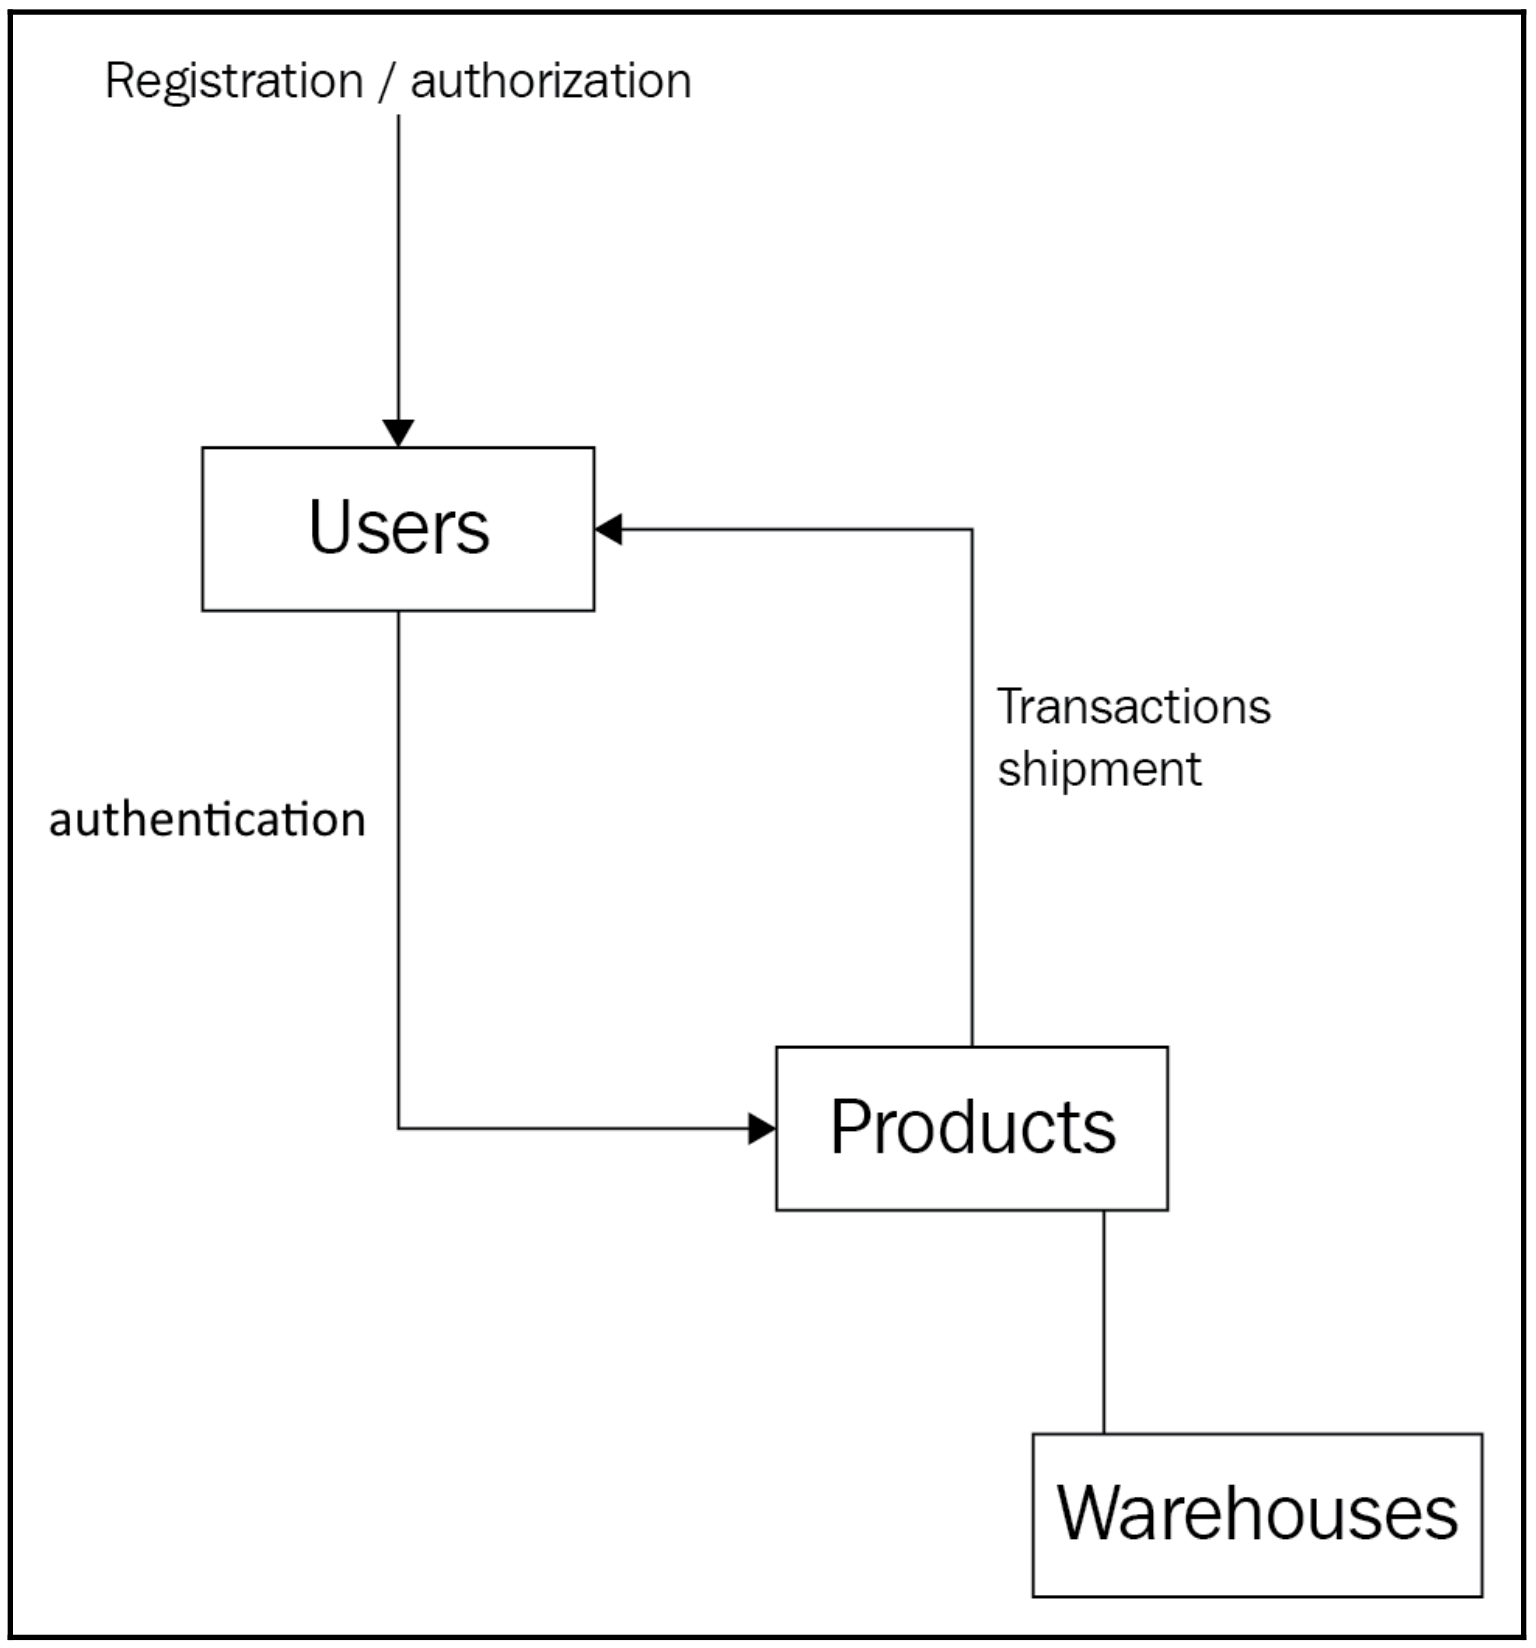
\includegraphics[width=0.6\textwidth]{content/Section-2/Chapter-10/1}
\end{center}

把实体和过程分解成类,它们之间的相互交流就是一门艺术,需要耐心和一致性。例如,我们尝试添加用户实体的详细信息。如创建规范步骤中所述,注册用户应该提供送货地址、电子邮件地址和信用卡详细信息。让我们画一个表示用户的类图: \par

\begin{center}
	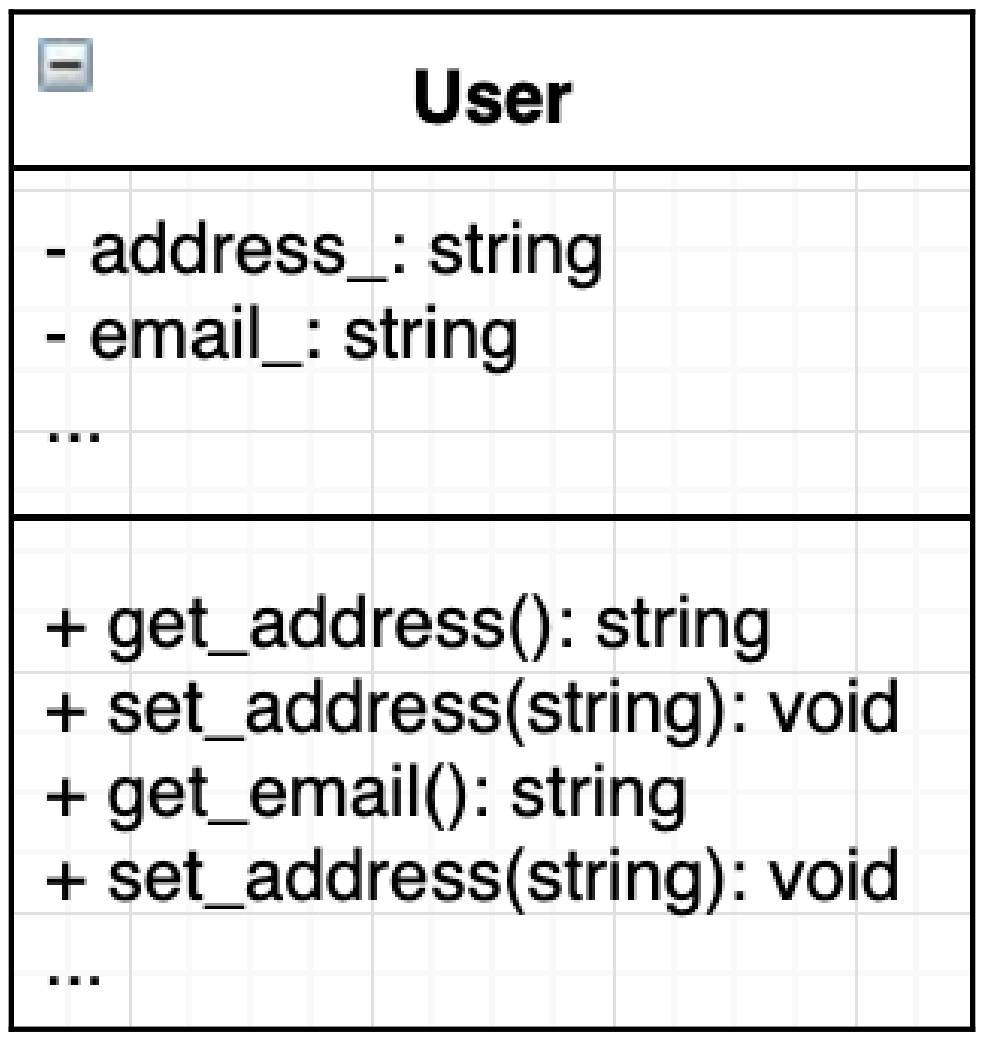
\includegraphics[width=0.4\textwidth]{content/Section-2/Chapter-10/2}
\end{center}

有一个有趣的问题:我们如何处理复杂类型?例如,用户的投递地址是复杂类型。它不可能只是字符串,因为我们可能需要根据用户的送货地址进行排序,以实现最佳的发货顺序。如果用户的送货地址与包含购买产品的仓库地址在不同的国家,那么货运公司可能会让我们(或用户)花费一大笔钱。这是一个很好的场景,它引入了一个新的问题,并更新了我们对项目的理解。当用户订购的产品分配到离用户很远的仓库时,我们应该处理这种情况。如果我们有很多仓库,我们应该选择一个距离用户最近的。这些问题不能马上得到具体的回答,但这可以保证项目的高质量。否则,这些问题就会在编码过程中出现,我们困在这些问题上的时间,就要比我们想象的要长。 \par
现在,如何将用户地址存储在User类中?一个简单的std::string就可以了,如下面的例子所示: \par

\begin{lstlisting}[caption={}]
class User
{
public:
	// code omitted for brevity
private:
	std::string address_;
	// code omitted for brevity
};
\end{lstlisting}

就其组件而言,地址是一个复杂的对象。地址可以包含国家名称、国家代码、城市名称和街道名称,甚至还可以包含纬度和经度。如果您需要找到离用户最近的仓库,那么越详细越好。制作更多类型,让程序员的设计更直观,这完全没有问题。例如,下面的结构体可能很适合描述用户的地址: \par

\begin{lstlisting}[caption={}]
struct Address
{
	std::string country;
	std::string city;
	std::string street;
	float latitude{};
	float longitude{};
};
\end{lstlisting}

现在,存储用户地址变得更加简单: \par

\begin{lstlisting}[caption={}]
class User
{
	// code omitted for brevity
	Address address_;
};
\end{lstlisting}
我们将在本章后面回到这个例子。 \par
设计项目的过程,可能需要有几个步骤重申项目需求。用前面的步骤澄清设计步骤之后,我们可以继续将项目分解为更小的组件,最好也都创建交互图。 \par
如下所示的交互图,将描述用户购买产品时所做的交易等操作: \par

\begin{center}
	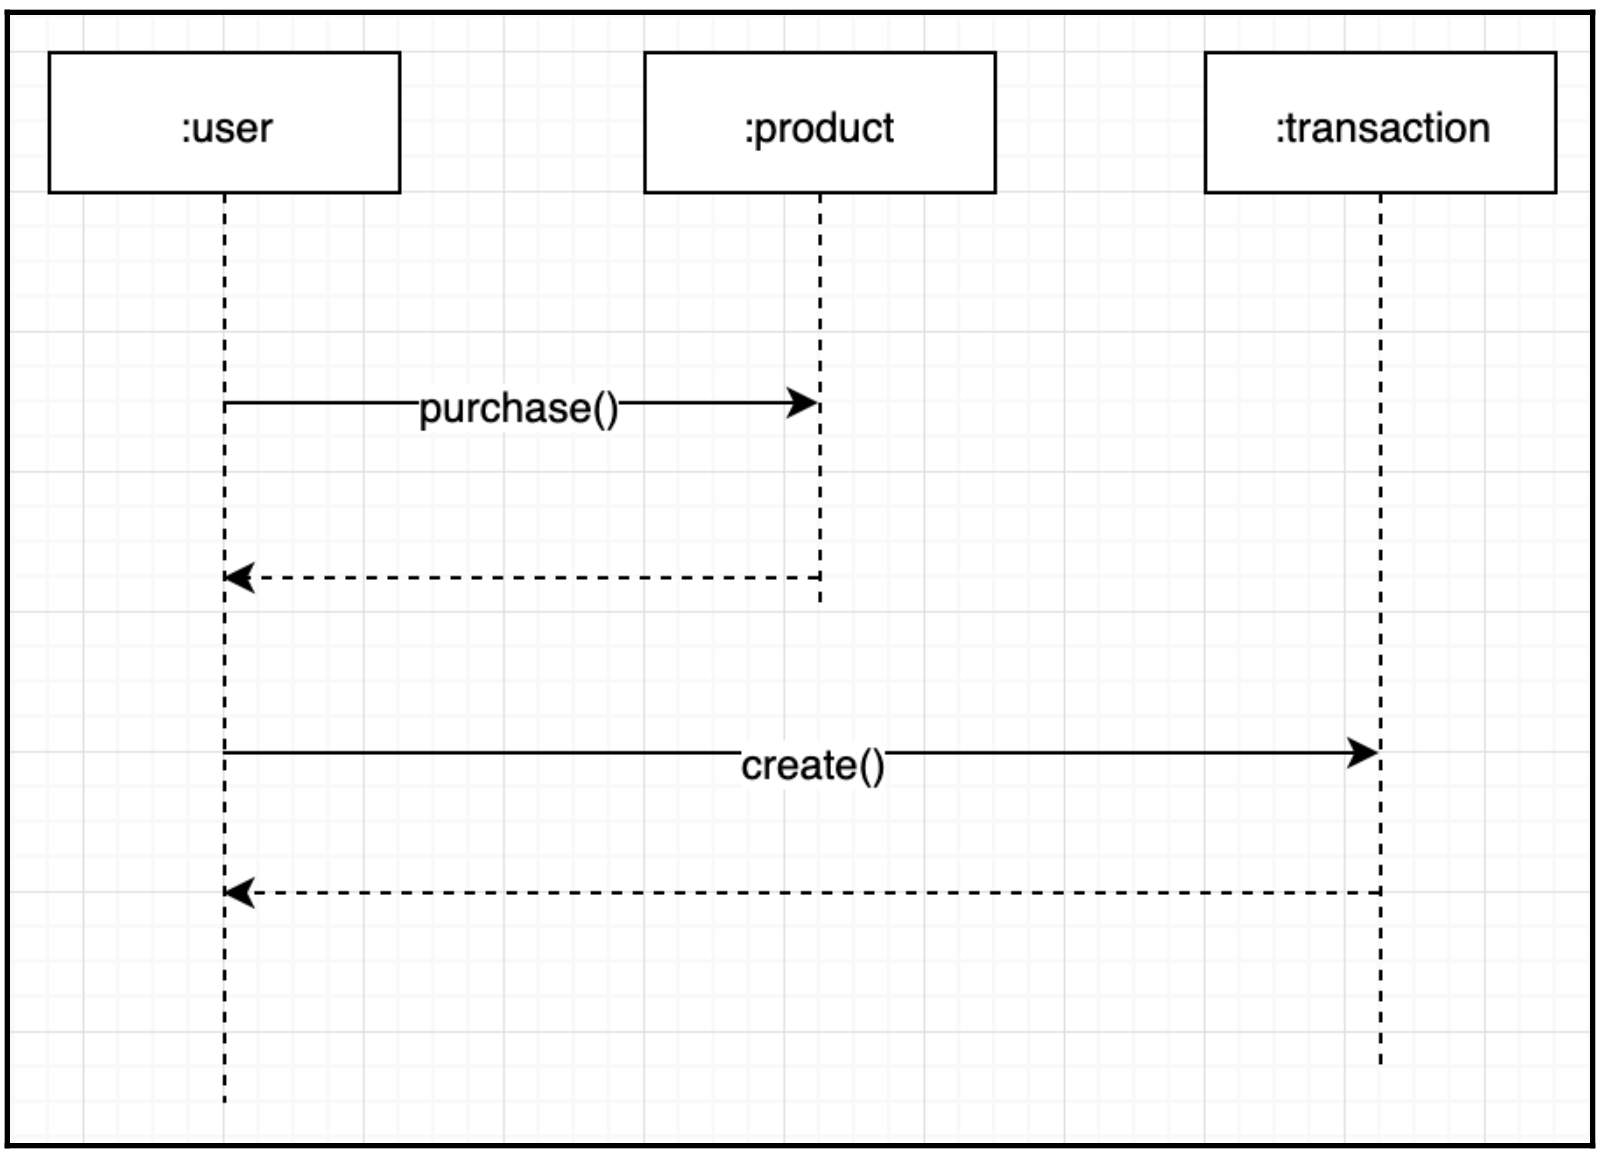
\includegraphics[width=0.6\textwidth]{content/Section-2/Chapter-10/3}
\end{center}

测试计划也可以认为是设计的一部分,包括如何测试最终应用程序的计划,例如:在此之前的步骤包括一个地址的概念,地址可以包含国家、城市等。正确的测试应该包括,检查是否可以在用户地址中成功设置国家。虽然测试计划通常不认为是开发者的任务,但对项目来说,它是一种很好的实践。在设计项目时,适当的测试计划将产生更多有用的信息。大多数输入数据处理和安全检查都在测试计划中发现,例如:在进行需求分析或编写功能规范时,对用户名或电子邮件地址设置严格的限制可能并不适用。测试计划会关注这样的场景,并迫使开发人员进行数据检查。然而,大多数开发人员并没有耐心做这些,而是直接进入项目开发的下一个步骤——编码。 \par

\noindent\textbf{}\ \par
\textbf{编码} \ \par

\noindent\textbf{}\ \par
\textbf{测试和稳定性} \ \par

\noindent\textbf{}\ \par
\textbf{发布和维护} \ \par

\noindent\textbf{}\ \par
\textbf{深入设计过程} \ \par

\noindent\textbf{}\ \par
\textbf{使用SOLID原则} \ \par

\noindent\textbf{}\ \par
\textbf{单一责任原则} \ \par

\noindent\textbf{}\ \par
\textbf{开闭原则} \ \par

\noindent\textbf{}\ \par
\textbf{里氏替换原则} \ \par

\noindent\textbf{}\ \par
\textbf{接口分离原则} \ \par

\noindent\textbf{}\ \par
\textbf{依赖倒置原则} \ \par

\noindent\textbf{}\ \par
\textbf{使用域驱动的设计} \ \par

\noindent\textbf{}\ \par
\textbf{利用设计模式} \ \par

\noindent\textbf{}\ \par
\textbf{库模式} \ \par

\noindent\textbf{}\ \par
\textbf{库模式} \ \par

\noindent\textbf{}\ \par
\textbf{库模式} \ \par

\noindent\textbf{}\ \par
\textbf{工厂模式} \ \par

\noindent\textbf{}\ \par
\textbf{总结} \ \par

\noindent\textbf{}\ \par
\textbf{问题} \ \par
\begin{enumerate}
	\item TDD的好处是什么?
	\item UML中交互图的目的是什么?
	\item 合成和聚合有什么区别?
	\item 如何描述里氏替换原则?
	\item 让我们假设给您一个类Animal和一个类Monkey。后者描述的是一种特殊的在树上跳的动物。从动物类继承猴子类是否违背开闭原则?
	\item 在本章讨论的Product类及其子类上应用工厂模式。
\end{enumerate}

\noindent\textbf{}\ \par
\textbf{扩展阅读} \ \par
更多资料请参阅: \par
\begin{itemize}
	\item Object-Oriented Analysis and Design with Applications by Grady Booch,  https:/​/www.​amazon.​com/​Object-​Oriented-​Analysis-​Design-​Applications-​3rd/​dp/	020189551X/​
	\item Design Patterns: Elements of Reusable Object-Oriented Software by Erich Gamma et	al, https:/​/​www.​amazon.​com/​Design-​Patterns-​Elements-​Reusable-​Object-	Oriented/​dp/​0201633612/​
	\item Code Complete: A Practical Handbook of Software Construction by Steve McConnel, https://www.amazon.com/Code-Complete-Practical-Handbook-Construction/dp/0735619670/
	\item Domain-Driven Design: Tackling Complexity in the Heart of Software by Eric	Evans,  https:/​/​www.​amazon.​com/​Domain-​Driven-​Design-​Tackling-
	Complexity-​Software/​dp/​0321125215/
\end{itemize}

\newpage










